\documentclass[final]{beamer}
\usetheme{RJH}
\usepackage[orientation=landscape,size=a0,scale=1.4]{beamerposter}
\usepackage{tikz}
\usetikzlibrary{shapes,arrows,decorations.markings}
%\usepackage[orientation=landscape,height=1067mm,width=1524mm,scale=1.4,debug]{beamerposter}

\usepackage[absolute,overlay]{textpos}
\usepackage[numbers,compress]{natbib}
\usepackage{booktabs}
\usepackage{multirow}
\usepackage{array}
%\usepackage{wrapfig}
\usepackage{rotating}
\graphicspath{{Graphics/}}

% single line bib
% http://tex.stackexchange.com/a/5574
%\usepackage{paralist}
%\renewenvironment{thebibliography}[1]{%
%  \section*{\refname}%
%  \let\par\relax\let\newblock\relax%
%  \inparaenum[{[}1{]}]}{\endinparaenum}
%\renewcommand{\bibitem}[1]{\item}

\newcolumntype{C}[1]{>{\centering\arraybackslash} m{#1} }
\setlength{\TPHorizModule}{1cm}
\setlength{\TPVertModule}{1cm}
\newcommand{\subblock}[1]{\bigskip\textbf{#1}}

\title{Reliability of gamma activity during semantic integration}
\author{Jona Sassenhagen \and Phillip Alday}
\institute{University of Marburg}
\footer{}
%\footer{Live code at \url{https://github.com/jona-sassenhagen/phijona---gamma}}
\date{}

\begin{document}
\begin{frame}{} 	
\begin{textblock}{15}(1,0)
%\colorbox{white}{

\includegraphics[width=5in]{marburg-logo-blackwhite.eps}
%}
\end{textblock}


\begin{textblock}{45}(1,04.5)
\begin{block}{Motivation: Reproducibility of Results}
Recently, research on event-related spectral perturbations (ERSPs) has begun to focus on the gamma band of the human EEG. A number of recent studies have reported gamma effects for semantic integration (related to cloze probability in classical N400 paradigms) \cite{mellemfriedmanmedvedev2013a,wangzhubastiaansen2012a,penolazziangrillijob2009a,hagoort2008a,hagoorthaldbastiaansen2004a}, but the effects thus far have been far less consistent than previous findings in the lower frequency bands (cf.~\cite{bastiaansenhagoort2006a,heinetammhofmann2006a,rohmklimeschhaider2001a,davidsonindefrey2007a,roehmschlesewskybornkessel2004a}).
In line with recent concerns about the reliability of effects in the brain sciences \cite{vulharriswinkielman2009a,simmonsnelsonsimonsohn2011a,kilner2013a}, we performed a pseudo-jackknife replication meta-analysis of existing experimental data. 
% killner 2013
%\subblock{Title}
\end{block}

\begin{block}{Prior Research}
\begin{tabular}{p{10cm} l c c c }
Study & $\gamma$-Cond. & Time  & Space & Freq. \\
\midrule
\cite{mellemfriedmanmedvedev2013a} & & & &\\
\cite{wangzhubastiaansen2012a} & & & & \\
\cite{penolazziangrillijob2009a} & & & &\\ 
\cite{hagoort2008a} & & & & \\
\cite{hagoorthaldbastiaansen2004a} & & & & \\
\end{tabular}
\end{block}

\begin{block}{Method (Pseudo-Jackknife)}
% Define block styles
% http://www.texample.net/tikz/examples/simple-flow-chart/
\tikzstyle{decision} = [diamond, draw, fill=blue!20, 
    text width=4.5em, text badly centered, inner sep=0pt,node distance=10cm]
\tikzstyle{block} = [rectangle, draw, fill=blue!20, 
    text width=5em, text centered, rounded corners, minimum height=4em, node distance = 8cm]
\tikzstyle{pole} = [rectangle, draw, fill=red!20, 
    text width=5em, text centered, rounded corners, minimum height=4em, node distance = 8cm]
\tikzstyle{line} = [draw, ultra thick, postaction={decorate}
									   ]
%\tikzstyle{cloud} = [draw, ellipse,fill=red!20, node distance=3cm,minimum height=2em]
    
\begin{tikzpicture}[auto,decoration={markings,
								mark=at position 1 with {\arrow[scale=4,black]{latex'}};
								}]
    % Place nodes
    % example shapes: block, cloud, decision
    \node [pole] (init) {Start};
    \node [block,below of=init] (preproc) {Wavelet decomposition for all experiments};
    \node [block, below of=preproc] (foreach-outer) {For each experiment $i$ in set};
   	\node [block, below of=foreach-outer] (geteffects) {Find largest effect $e_i$ (time,space, frequency)};
	\node [block, right of=geteffects] (foreach-inner) {For each experiment $j$ in set};
	\node [block, right of=foreach-inner] (crosstest) {Test whether effect $e_i$ is significant in exp. $j$};
    \node [decision, right of=crosstest] (endfor-inner) {More exp. to crosstest?};
    \node [block, above of=crosstest] (forloop-inner) {Next exp. $j$};
    \node [decision, below of=geteffects] (endfor-outer) {More exp. to explore?};
    \node [block, left of=geteffects] (forloop-outer) {Next exp. $i$};
    \node [pole, below of=endfor-outer] (finish) {Stop}; 

    %\node [block, below of=] () {};
    % Draw edges
    \path [line] (init) -- (preproc);
    \path [line] (preproc) -- (foreach-outer);
    \path [line] (foreach-outer) -- (geteffects);
    \path [line] (geteffects) -> (foreach-inner);
    \path [line] (foreach-inner) -- (crosstest);
    \path [line] (crosstest) -- (endfor-inner);
    \path [line] (endfor-inner) |- node [near start] {yes} (forloop-inner);
    \path [line] (forloop-inner) -| (foreach-inner);
    \path [line] (endfor-inner) |- node {no} (endfor-outer);
    \path [line] (endfor-outer) -| node {yes} (forloop-outer);
    \path [line] (forloop-outer) |-  (foreach-outer);
	\path [line] (endfor-outer) -> node {no} (finish);
	
\end{tikzpicture}
\end{block}
\end{textblock}

\begin{textblock}{25}(20,35.5)
\begin{block}{Data}
\begin{itemize}
\item 11 Studies
\item 7 auditory, 4 visual presentation
\item 3 languages (German, Japanese, Welsh)
\end{itemize}
\end{block}
\end{textblock}

\begin{textblock}{63}(47.5,04.5)
\begin{block}{Replication}
%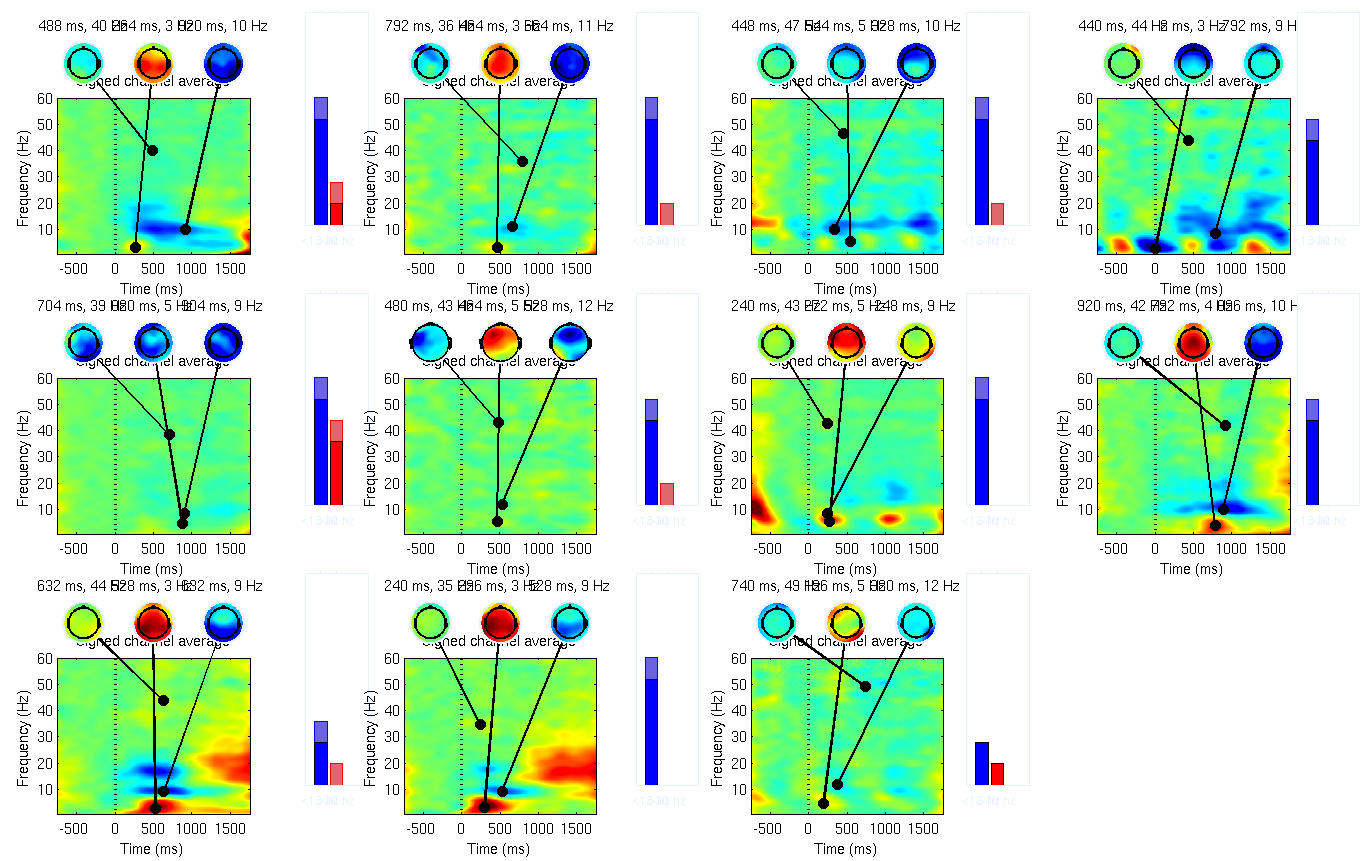
\includegraphics[height=73cm,width=70cm]{gamma}
\begin{tabular}{c c c}
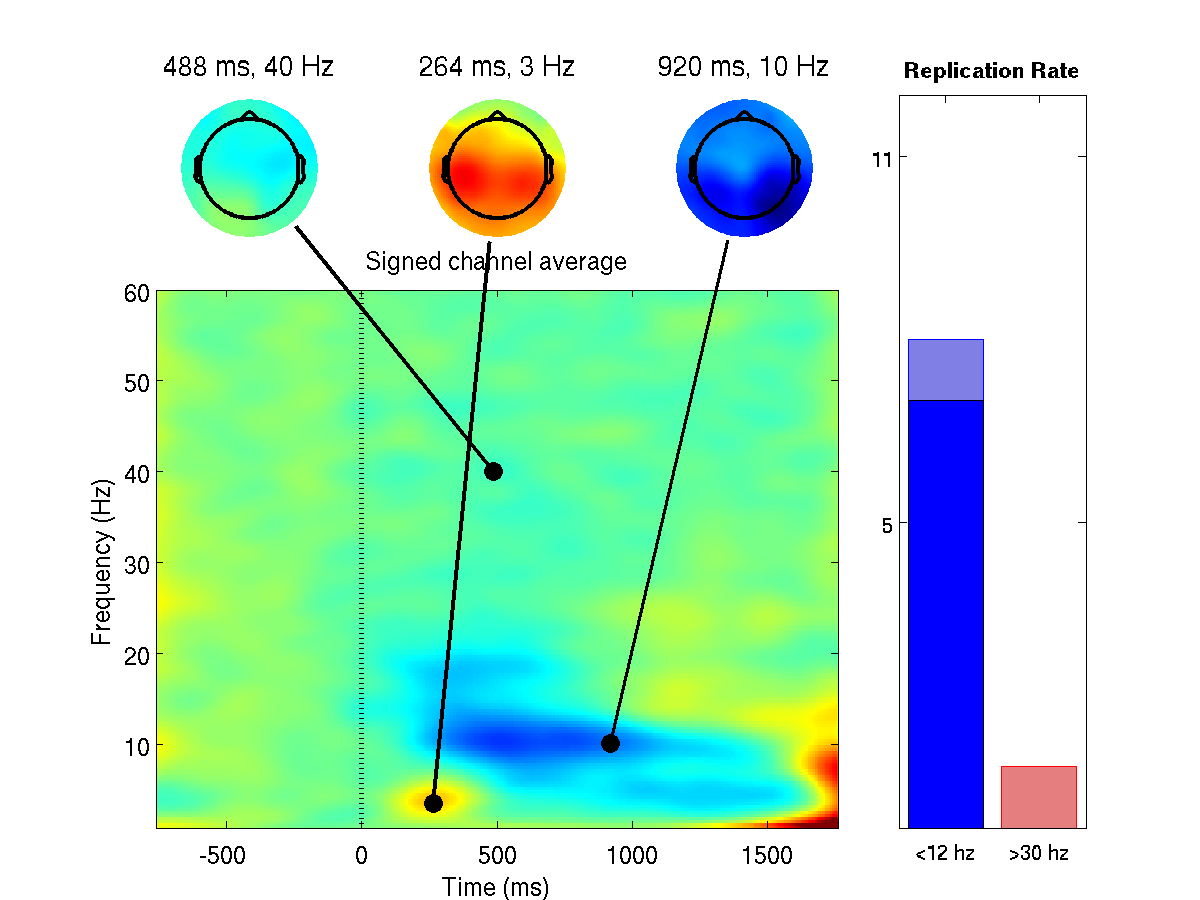
\includegraphics{gamma01} & 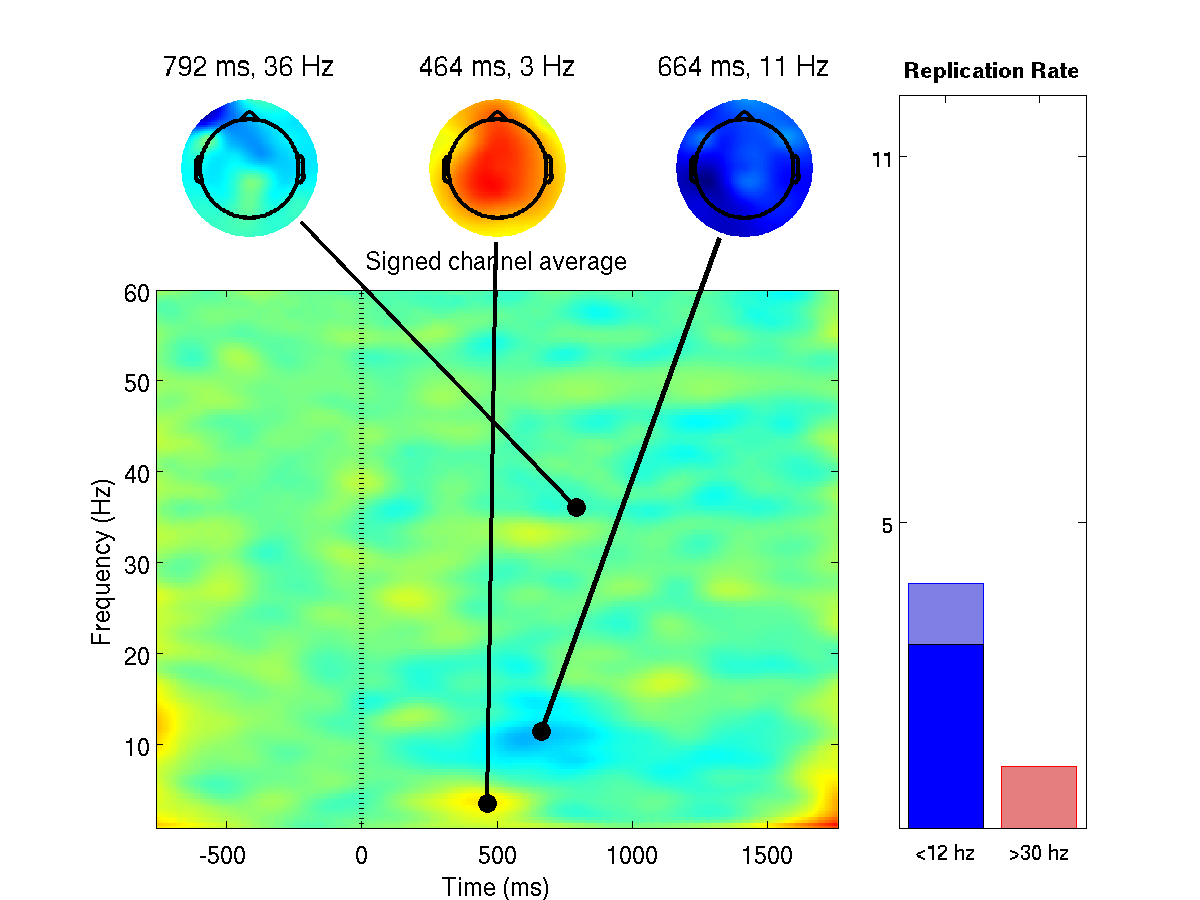
\includegraphics{gamma02} & 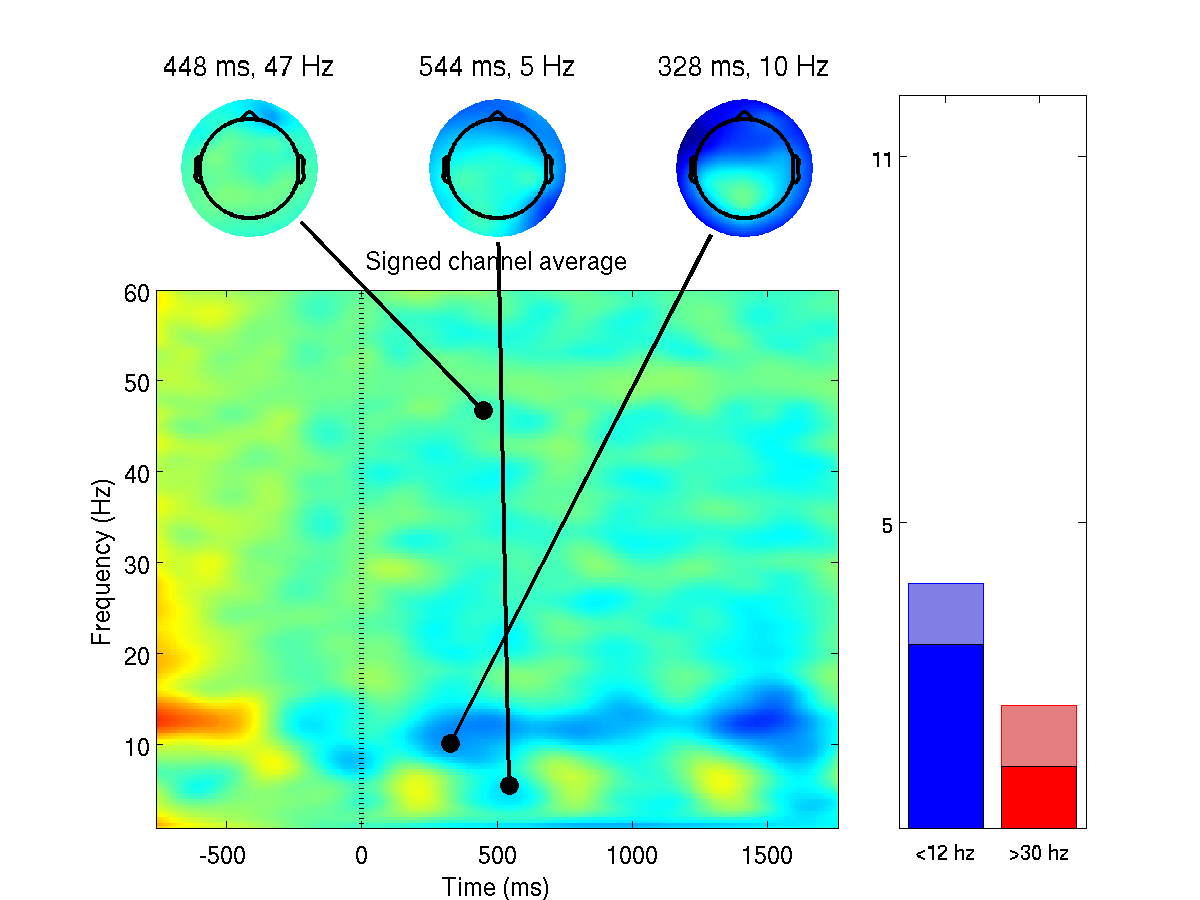
\includegraphics{gamma03} \\
DE / AUD / HIGH / SEM & DE / AUD / MED / COMP & DE / VIS / HIGH / PROBE \& ACC \\
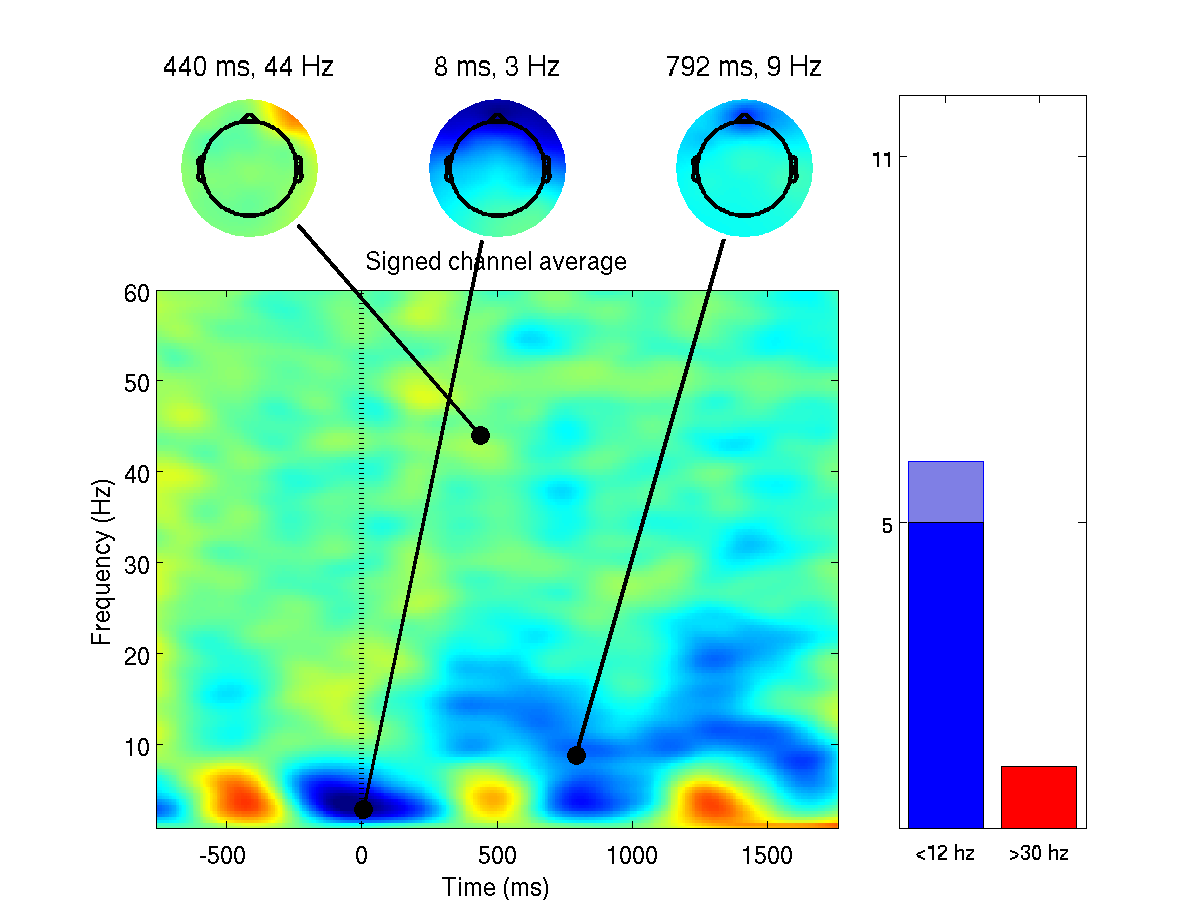
\includegraphics{gamma04} & 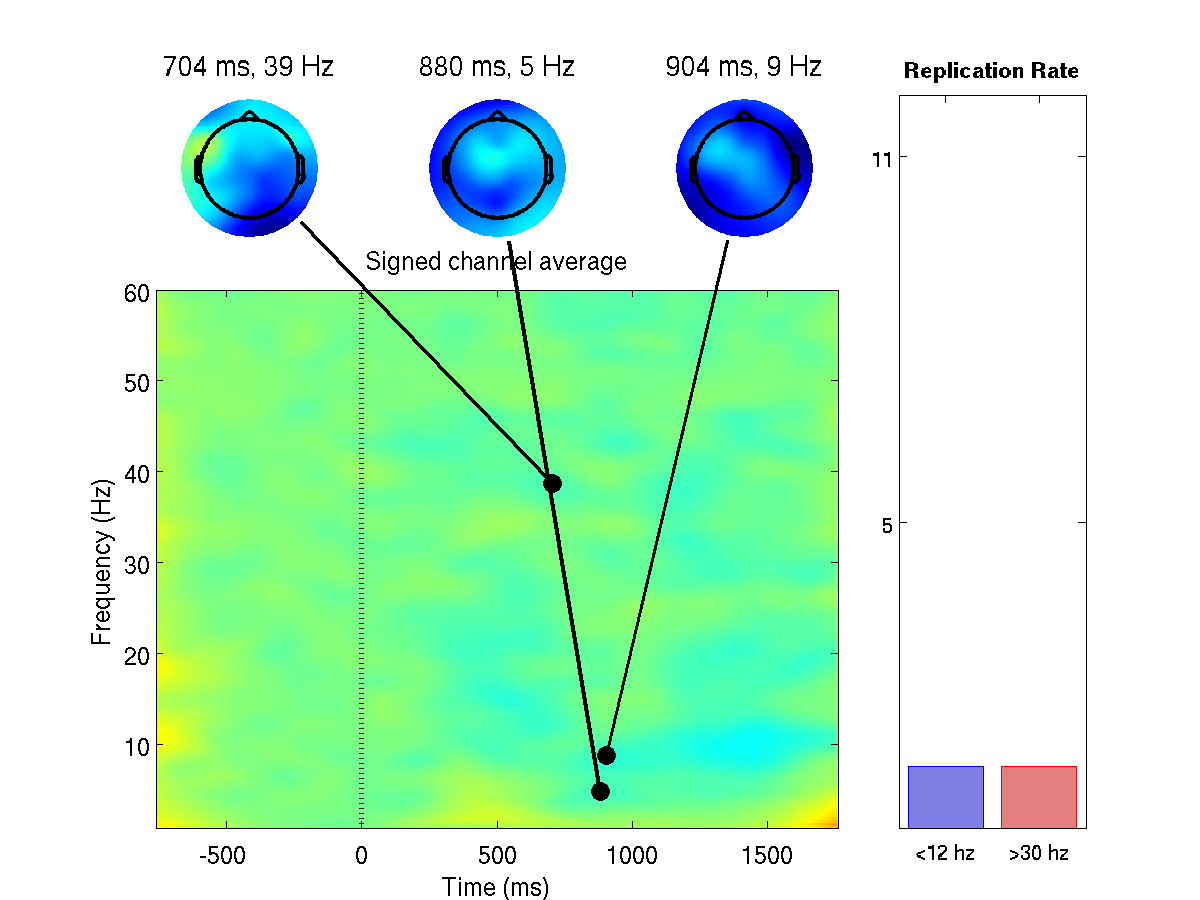
\includegraphics{gamma05} & 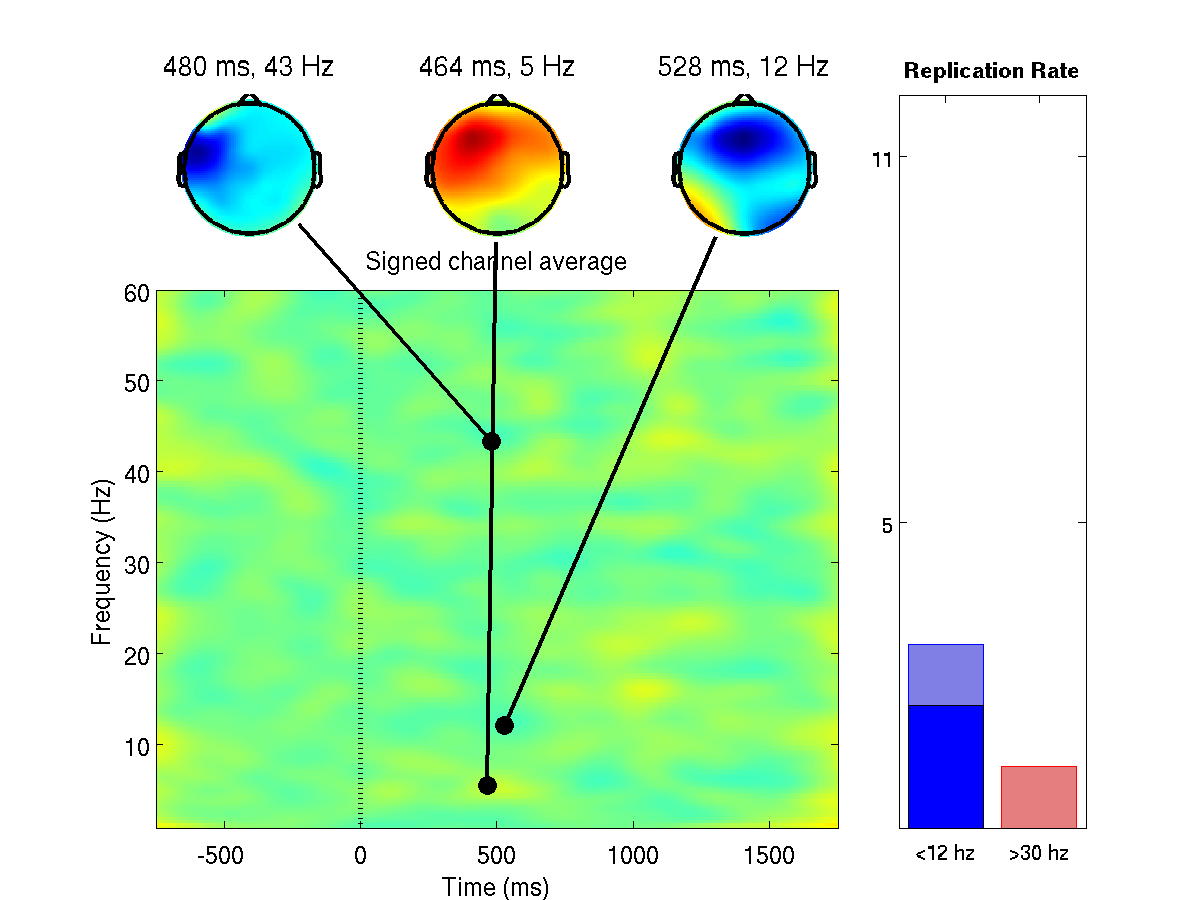
\includegraphics{gamma06} \\
DE / VIS / MED / PROBE \& ACC  & DE / VIS / MED / PASS & DE / VIS / MED / PASS \\
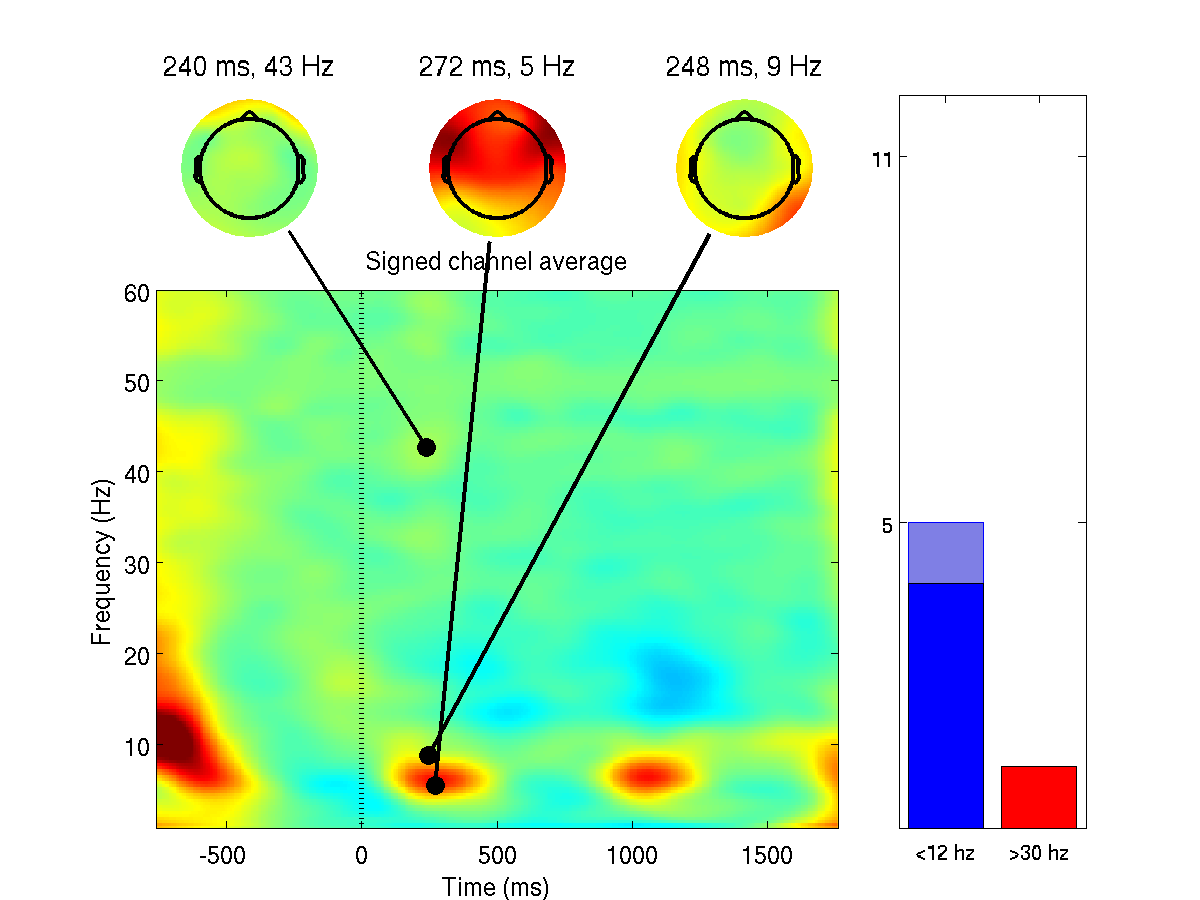
\includegraphics{gamma07} & 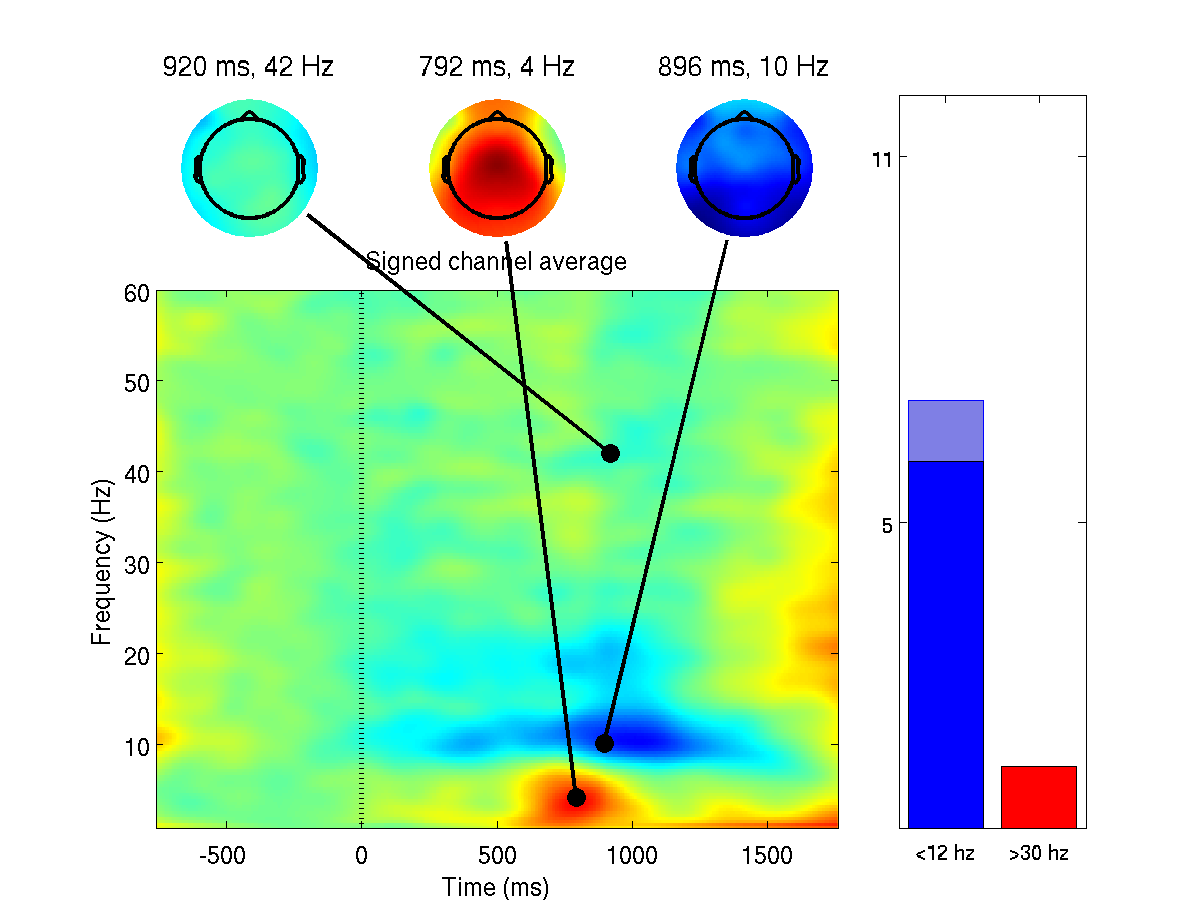
\includegraphics{gamma08} & 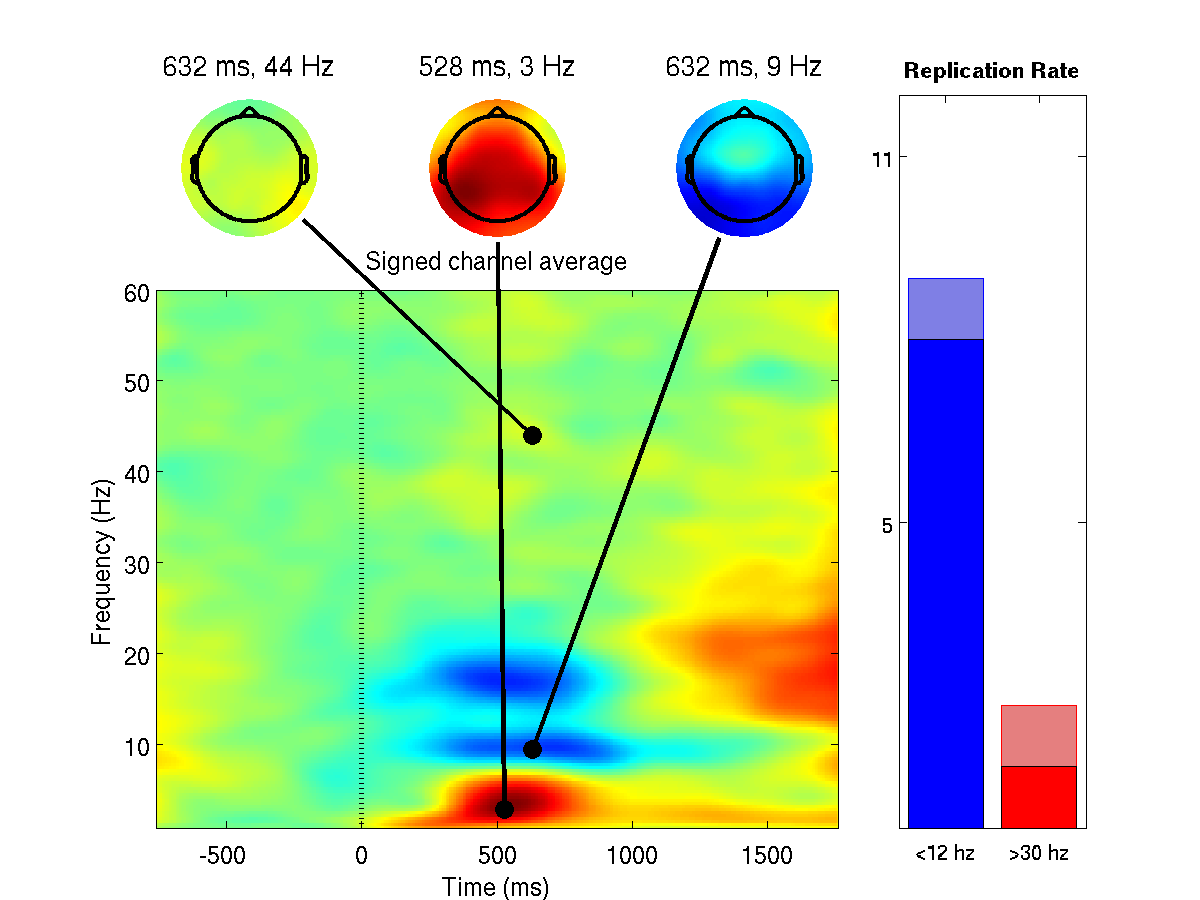
\includegraphics{gamma09} \\
JA / VIS / MED / PROBE & DE / AUD / MED / SEM  & DE / AUD / MED / SEM \\
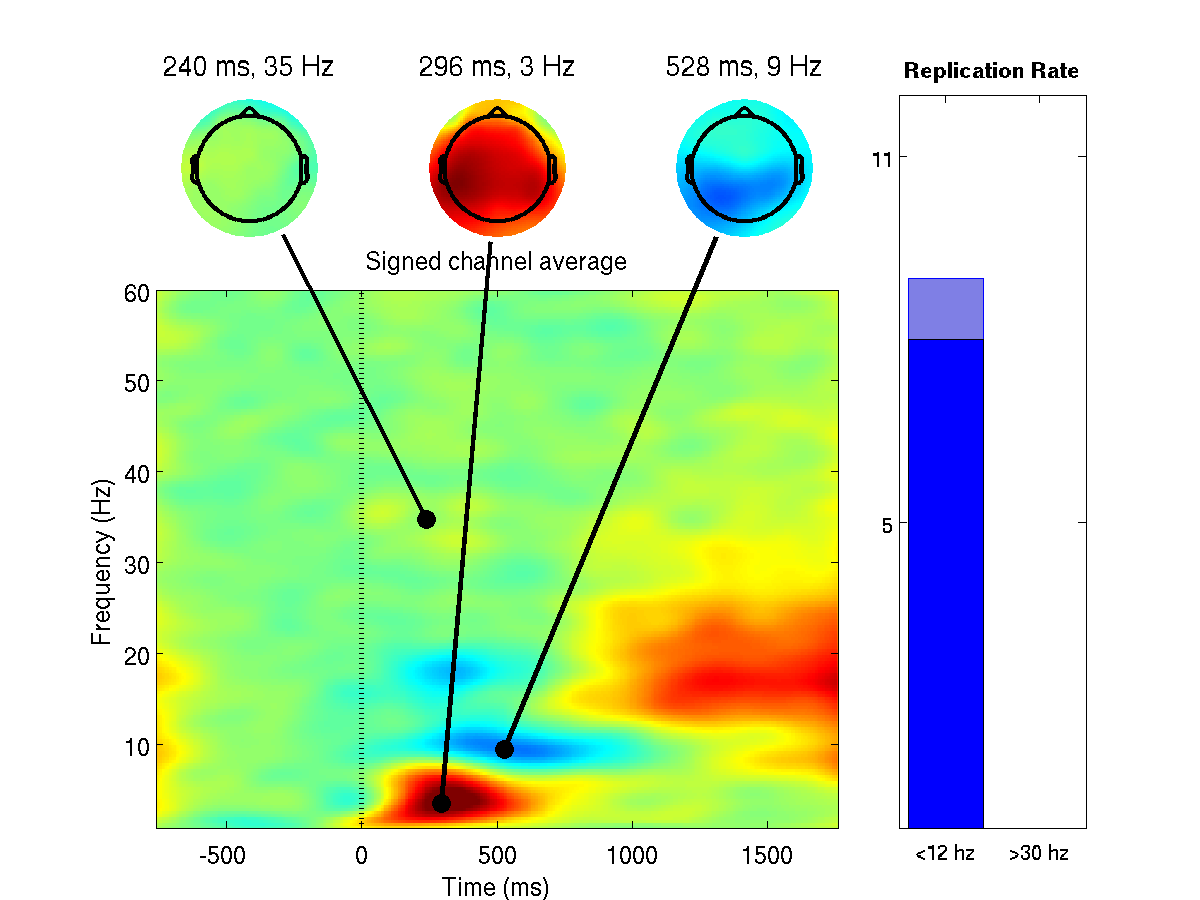
\includegraphics{gamma10} & 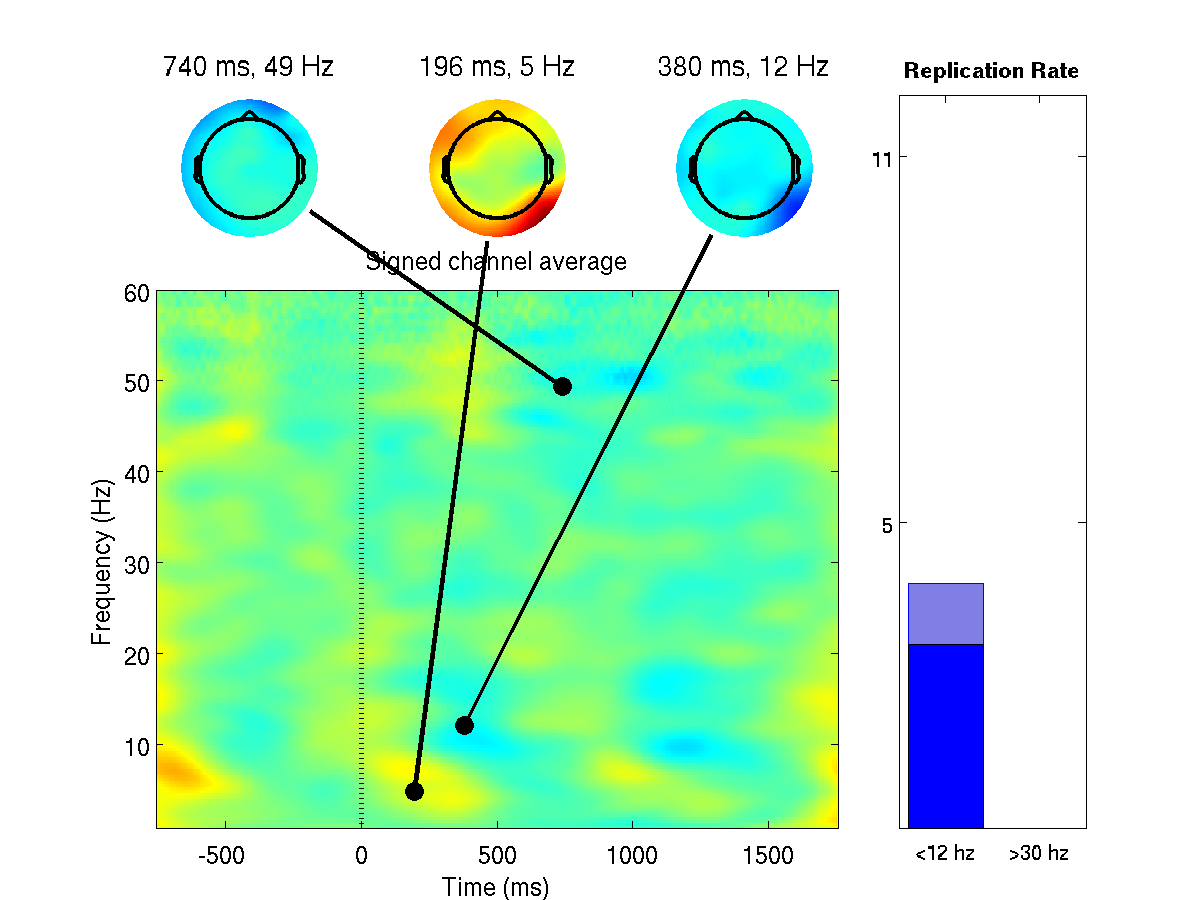
\includegraphics{gamma11} &  \\
DE / AUD /HIGH / SEM & CY / VIS / MED / PROBE \& ACC &  \\
%German - visual & German auditory & English visual & English auditory \\ 
\end{tabular}
\end{block}
HIGH, MED, LOW = high, medium, low close probability 

SEM = semantic judgment; COMP = comprehension task; PROBE = probe task; \\ ACC = acceptability judgment task; PASS = passive listening 
\end{textblock}

\begin{textblock}{8}(110.5,04.5)

\end{textblock}

% like 2012
%\begin{textblock}{27.5}(90,58.7)
% long on the bottom
%\begin{textblock}{95}(20.5,75.7)
\begin{textblock}{15.5}(102,58.7)
\begin{block}{Literature}
\tiny
\bibliographystyle{poster}
\bibliography{poster.bib}
\end{block}
\end{textblock}

\begin{textblock}{10}(113,69.5)
%\includegraphics[width=2in]{contactinfo-qrcode.png}
\end{textblock}
\begin{textblock}{10}(113,75.5)
%\includegraphics[width=2in]{code-qrcode.png}
\end{textblock}

\end{frame}
\end{document}
